\definecolor{blue}{rgb}{0.2,0.5,0.8}
\section{Ground segment}
The ground segment is composed by the Ground Stations (GS) and the Mission Control Center (MCC), that allow the receiving of the information from the constellation to the Earth.\\
The placement of the different nodes of the Ground Segment is shown in the following map.  
\begin{figure}[H]
\begin{center}
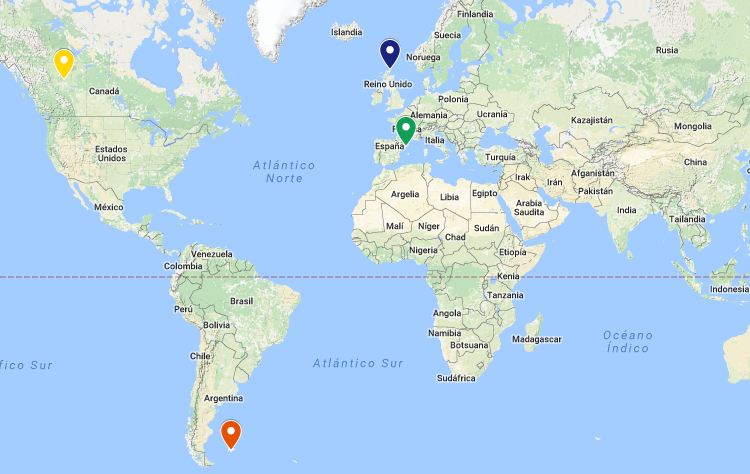
\includegraphics[scale=0.6]{map.PNG} 
\caption{Location of the GS and MCC}
\end{center}
\end{figure}
\begin{table}[H]
\begin{center}
\begin{tabular}{|c|c|c|}
\hline
\rowcolor{blue} \textbf{Node}&\textbf{Color in the map}&\textbf{Country}\\
\hline
GS1&Yellow&Canada\\
\hline
GS2&Orange&Falkland Islands\\
\hline
GS3&Blue&United Kingdom\\
\hline
MCC&Green&Spain\\
\hline
\end{tabular}
\caption{Countries of location}
\end{center}
\end{table}
The MCC is composed by a set of offices with good connection to the GS. The systems that compose the GS are exposed in the following table. 
\begin{table}[H]
\begin{center}
\begin{tabular}{|p{4cm}|p{4cm}|p{4cm}|p{4cm}|}
\hline
\rowcolor{blue} \textbf{System}&\textbf{Features}&\textbf{Purpose}&\textbf{Elements included}\\
\hline
S-band&Half-duplex system: downlink and uplink capability&Housekeepink data/TT\& C \newline
Client data upload&
Transciever 
\newline
LNA
\newline
HPA
\newline
RF Limiter
\newline
RF Swith
\newline
RF Fuse
\newline
Rotors\\
\hline
X-band&X-band downlink capacity&Client data download&X-band receiver
\newline
LNA
\newline
RF Limiter
\newline
RF Fuse
\newline
Rotor\\
\hline
\end{tabular}
\caption{GS's systems}
\end{center}
\end{table}